\documentclass{article}

\usepackage{graphicx}
\usepackage{amsmath}
\usepackage{fancyhdr}
\usepackage{float}
\usepackage{titlesec}
\usepackage{verbatim}
\usepackage{fancyvrb}
\usepackage[dvipsnames]{xcolor}
\usepackage[sorting=none]{biblatex}
\usepackage[margin=1in]{geometry}
\usepackage[font={small,it}]{caption}
\usepackage{placeins}
\usepackage{xepersian}


%%%%txt
\RecustomVerbatimCommand{\VerbatimInput}{VerbatimInput}%
{fontsize=\footnotesize,
 %
 frame=lines,  % top and bottom rule only
 framesep=2em, % separation between frame and text
 rulecolor=\color{Gray},
 %
 label=\fbox{\color{Black}txt file},
 labelposition=topline,
 %
 commandchars=\|\(\), % escape character and argument delimiters for
                      % commands within the verbatim
 commentchar=*        % comment character
}
%%%%txt


%\DeclareMathOperator*{\btie}{\bowtie}
\addbibresource{bibliography.bib}
\settextfont[Scale=1.2]{B-NAZANIN.TTF}
\setlatintextfont[Scale=1]{Times New Roman}
\renewcommand{\baselinestretch}{1.5}
\pagestyle{fancy}
\fancyhf{}
\rhead{تکلیف پنجم آزمایشگاه شبکه ‌های کامپیوتری}
\lhead{\thepage}
\rfoot{علیرضا ابره فروش}
\lfoot{9816603}
\renewcommand{\headrulewidth}{1pt}
\renewcommand{\footrulewidth}{1pt}

\begin{document}
\begin{titlepage}
\begin{center}

\includegraphics[width=0.4\textwidth]{figures/IUT Logo.png}\\
        
\LARGE
\textbf{دانشگاه صنعتی اصفهان}\\
\textbf{دانشکده مهندسی برق و کامپیوتر}\\
        
\vfill
        
\huge
\textbf{عنوان: تکلیف چهارم درس ریزپردازنده}\\
        
\vfill
        
\LARGE
\textbf{نام و نام خانوادگی: علیرضا ابره فروش}\\
\textbf{شماره دانشجویی: 9816603}\\
\textbf{نیم\,سال تحصیلی: پاییز 1400}\\
\textbf{مدرّس: دکتر عارف کریمی افشار}\\
\end{center}
\end{titlepage}


%\tableofcontents
\newpage



\section{}%1
ابتدا دیوایس‌های شبکه را کنار هم به شکل زیر می‌چینیم.

\begin{figure}[H]
    \centering
    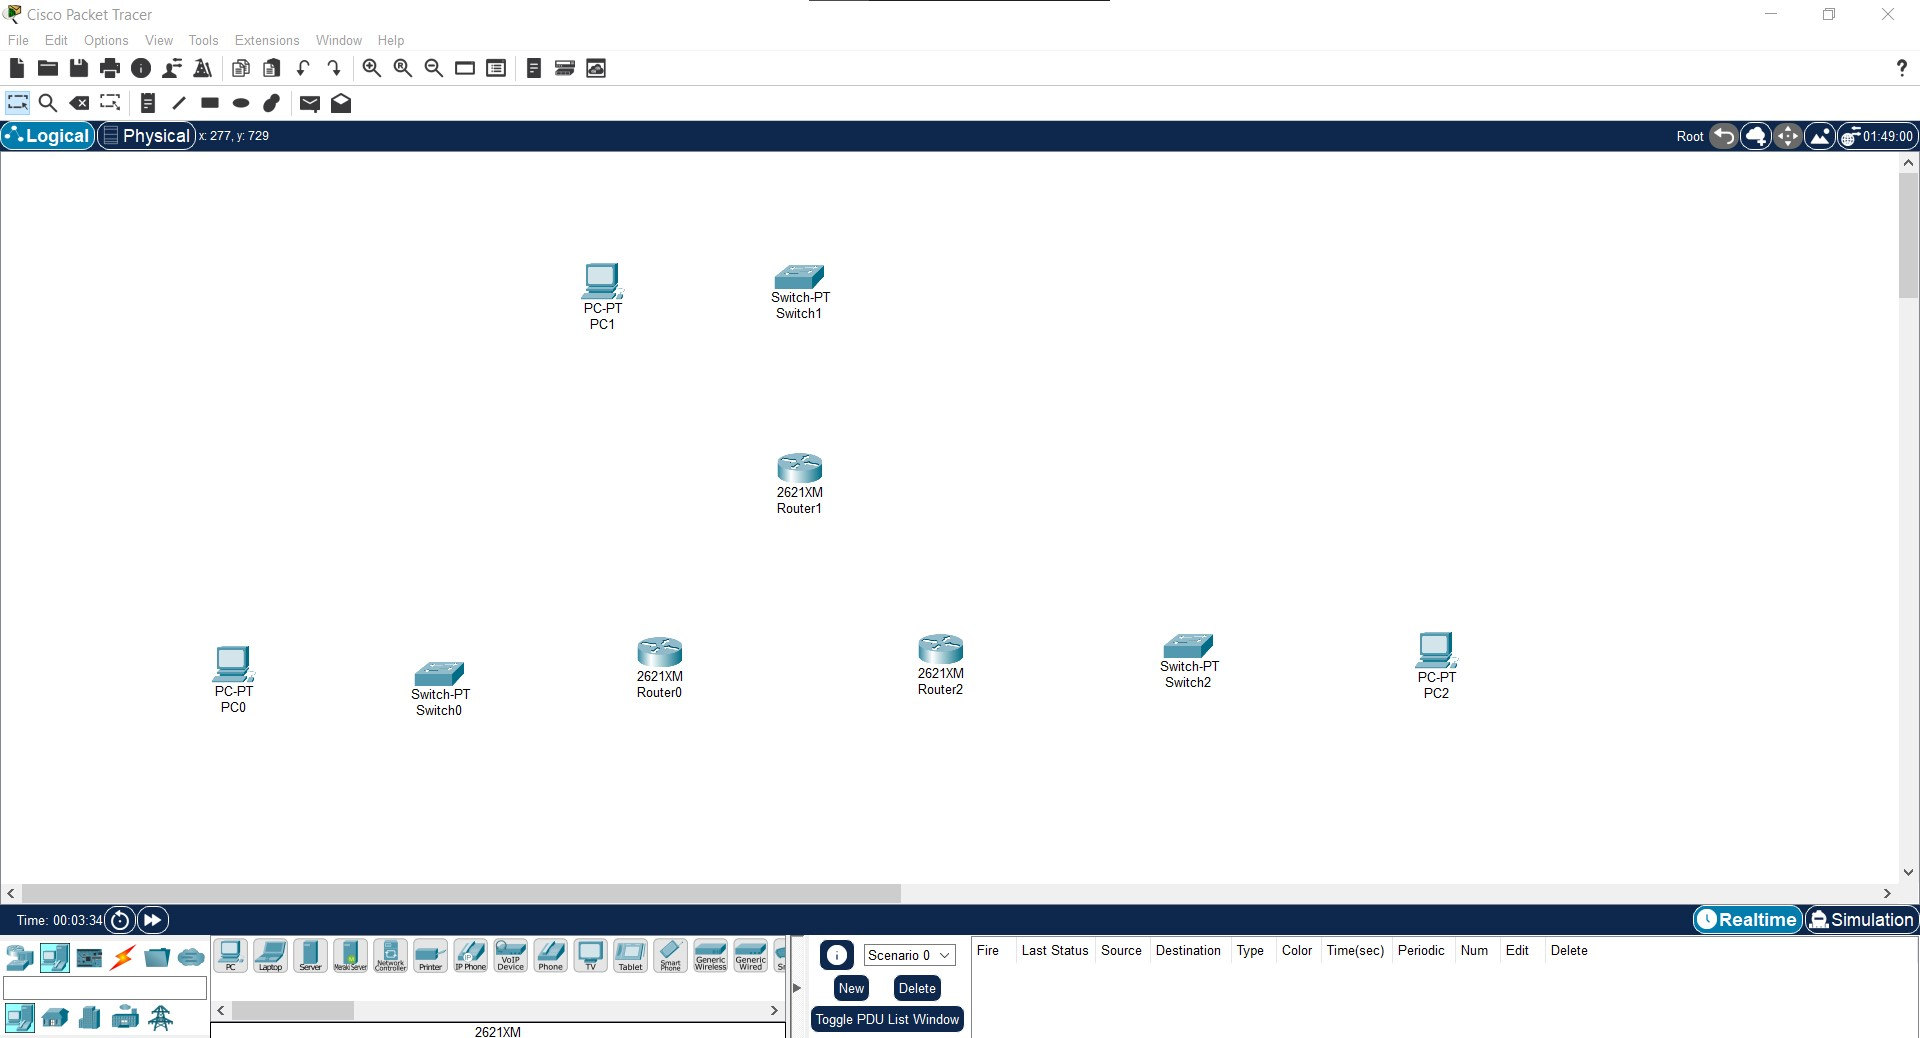
\includegraphics[width=1.0\textwidth]{figures/1.jpg}
    \caption{}
    \label{fig:fig1}
\end{figure}
سپس اتصالات را در حالت پیش‌فرض برقرار می‌کنیم.
\begin{figure}[H]
    \centering
    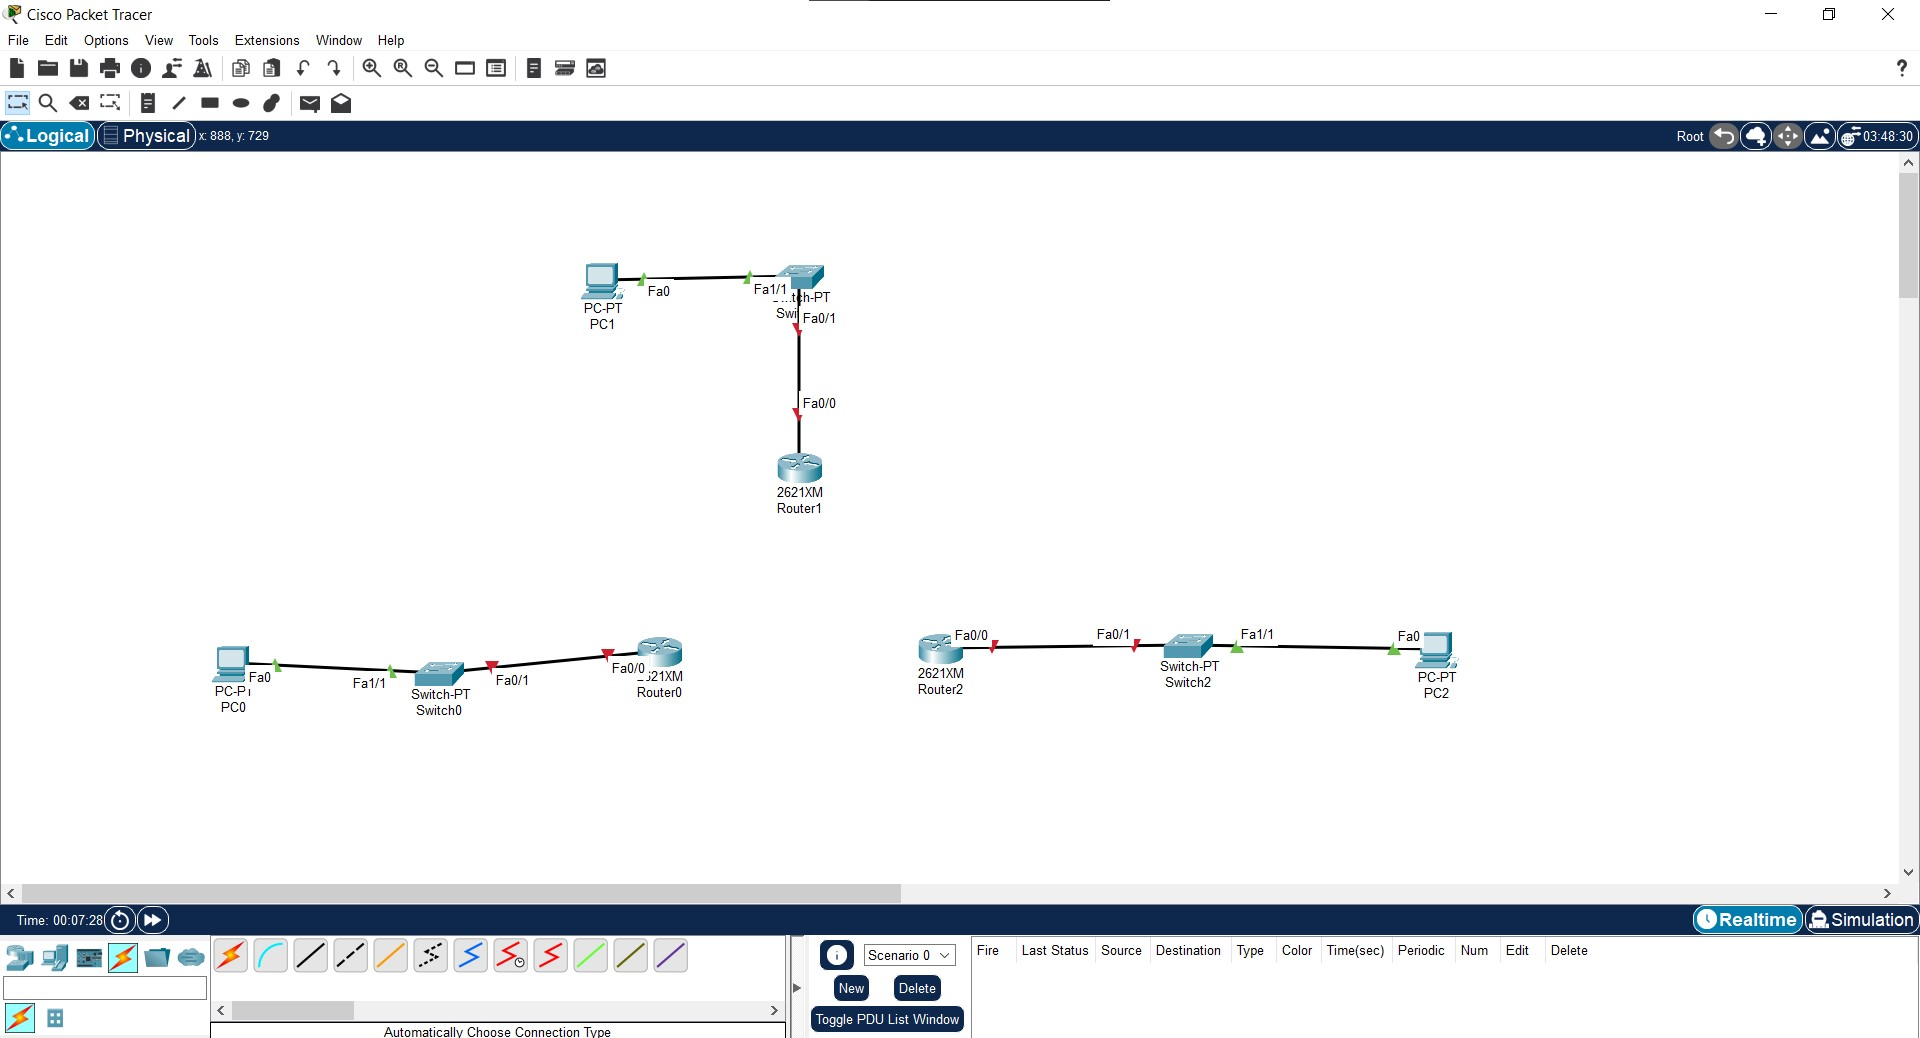
\includegraphics[width=1.0\textwidth]{figures/2.jpg}
    \caption{}
    \label{fig:fig1}
\end{figure}
برای اتصال سریال در روترها باید \lr{WIC-2T} به روتر به شکل زیر اضافه شود. توجه شود که روتر را ابتدا باید خاموش کنیم.
\begin{figure}[H]
    \centering
    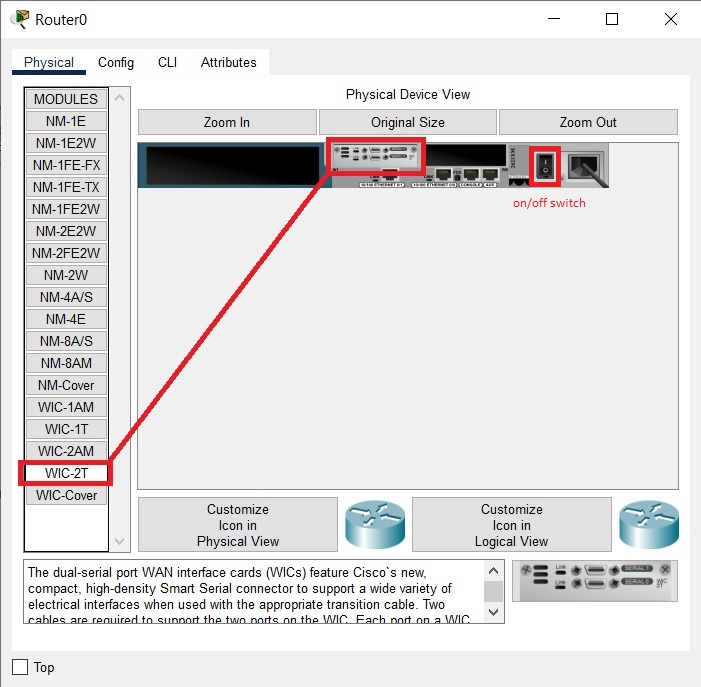
\includegraphics[width=0.75\textwidth]{figures/3.jpg}
    \caption{}
    \label{fig:fig1}
\end{figure}
روترها را در حالت پیش‌فرض به یکدیگر متصل می‌کنیم.
\begin{figure}[H]
    \centering
    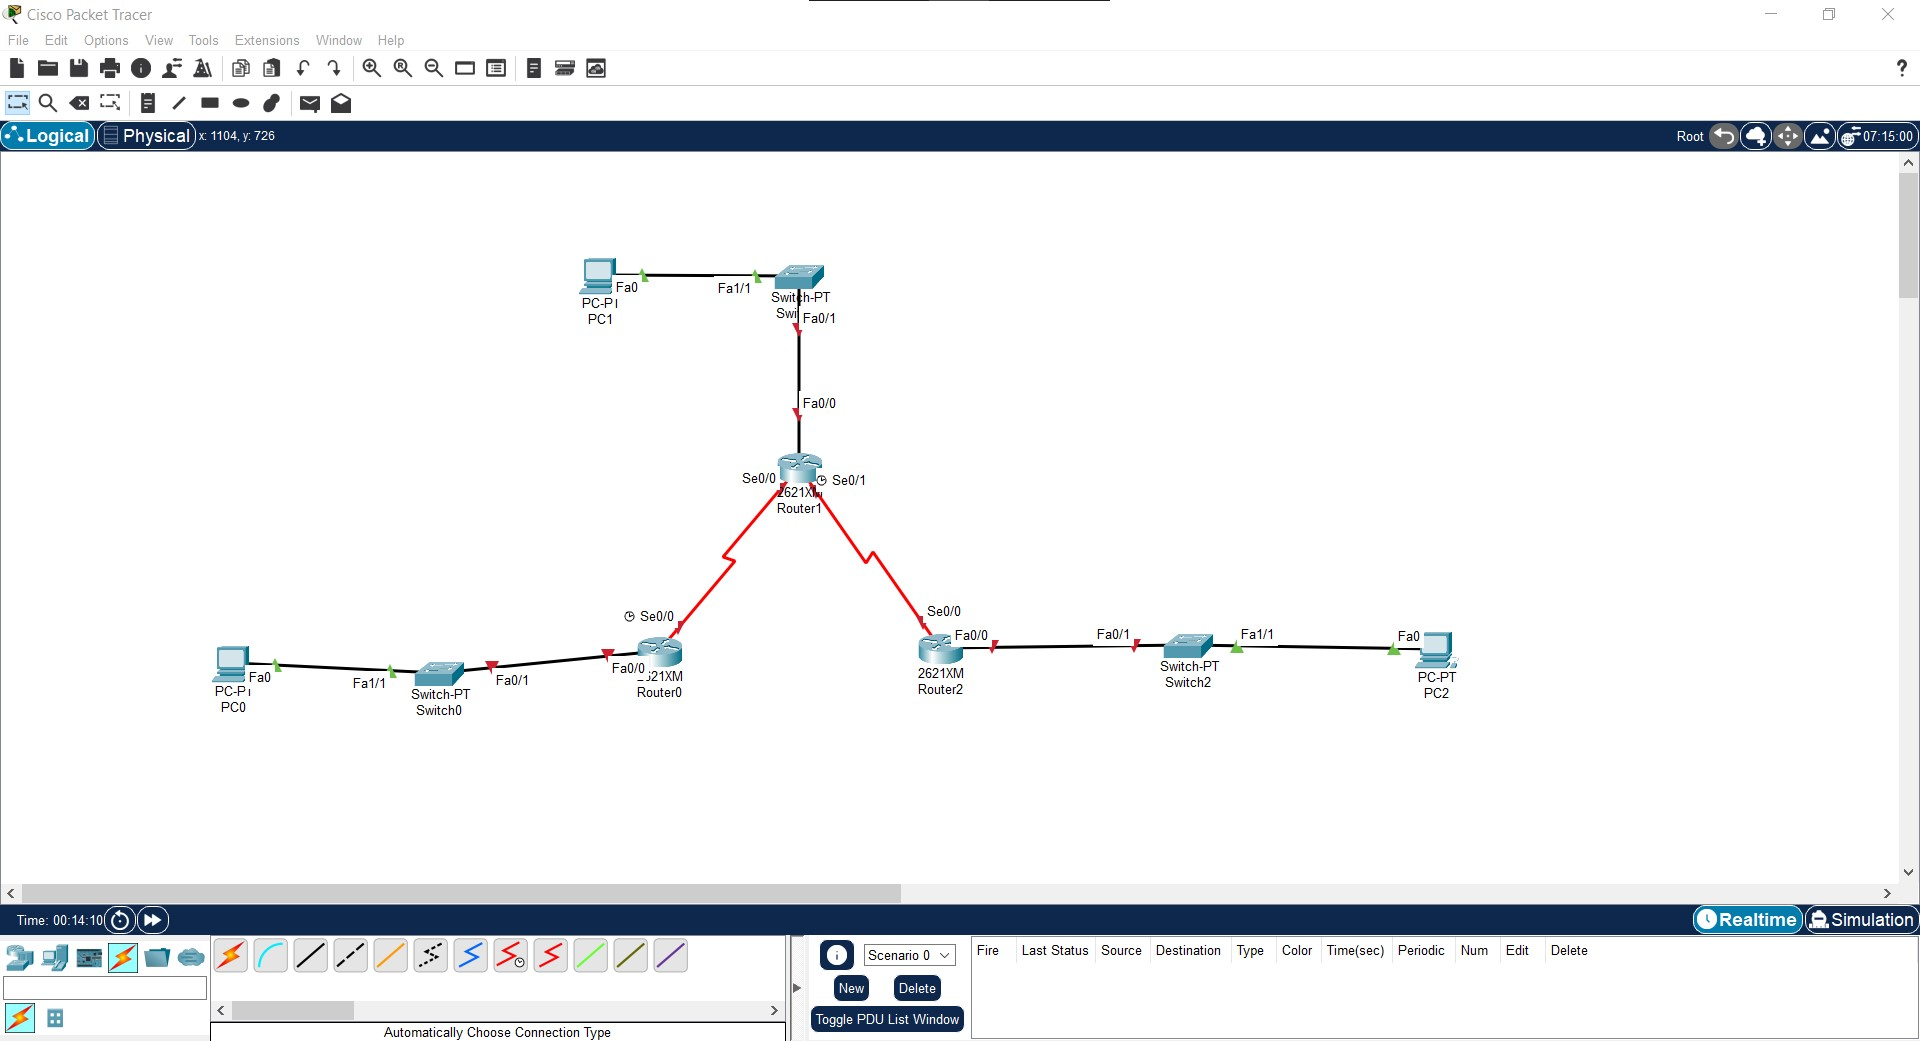
\includegraphics[width=1.0\textwidth]{figures/4.jpg}
    \caption{}
    \label{fig:fig1}
\end{figure}








\section{}%2
به شکل زیر می‌توانیم نام مسیریاب را تغییر دهیم.
\begin{figure}[H]
    \centering
    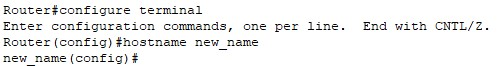
\includegraphics[width=0.5\textwidth]{figures/28.jpg}
    \caption{}
    \label{fig:fig1}
\end{figure}


\section{}%3
به شکل زیر برای ورود به حالت \lr{Privilage} رمز عبور تعیین می‌کنیم.
\begin{figure}[H]
    \centering
    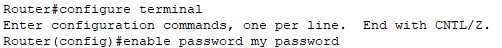
\includegraphics[width=0.5\textwidth]{figures/29.jpg}
    \caption{}
    \label{fig:fig1}
\end{figure}


\section{}%4
روتر 0 را به شکل زیر کانفیگ می‌کنیم. توجه شود که برای کانفیگ روتر، روتر حتما باید روشن باشد. کلاک‌ریت تنها به یکی از سرهای اینتفیس سریال (سر دارای ساعت) داده می‌شود.
\begin{figure}[H]
    \centering
    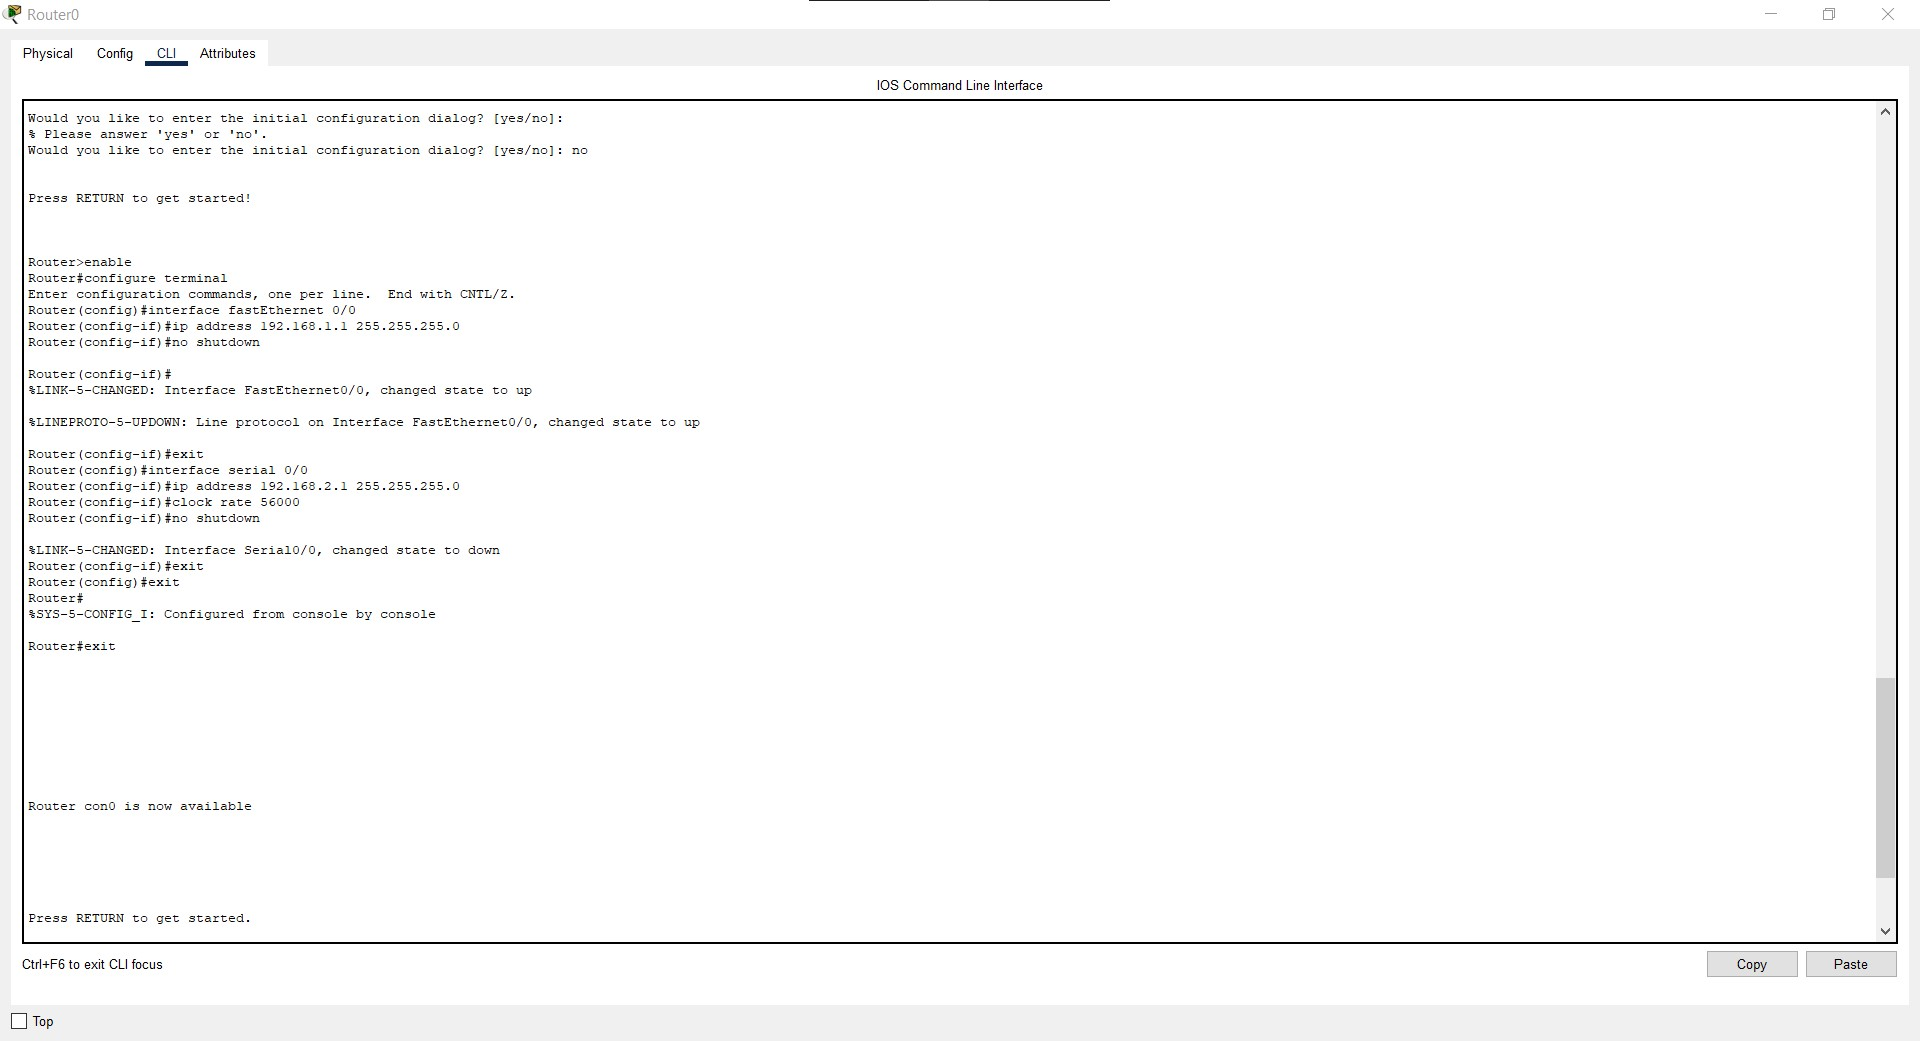
\includegraphics[width=1.0\textwidth]{figures/5.jpg}
    \caption{}
    \label{fig:fig1}
\end{figure}
می‌بینیم که روتر 0 کانفیگ شده است.
\begin{figure}[H]
    \centering
    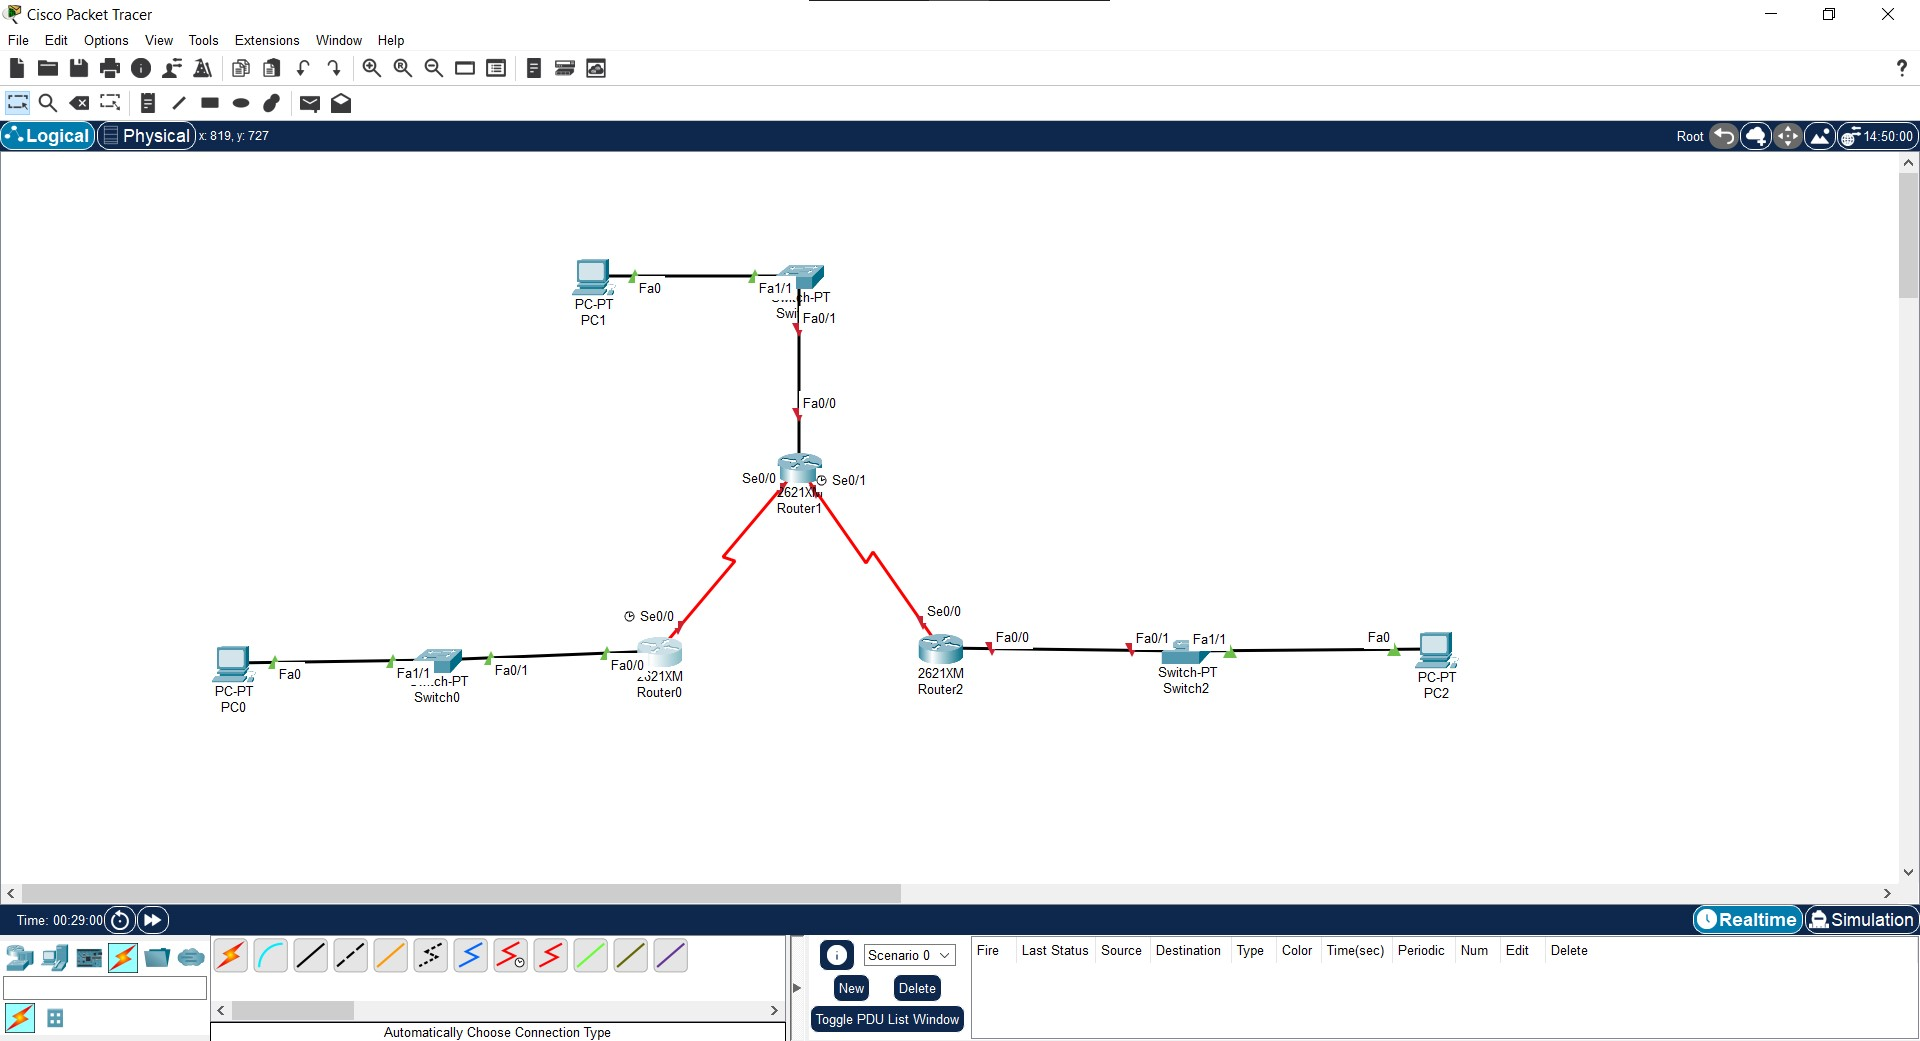
\includegraphics[width=1.0\textwidth]{figures/6.jpg}
    \caption{}
    \label{fig:fig1}
\end{figure}
بقیه‌ی روترها هم به همین شکل با آدرس‌های مربوطه کانفیگ می‌شوند. در نهایت اتصال در شبکه به شکل زیر به طور کامل برقرار است.
\begin{figure}[H]
    \centering
    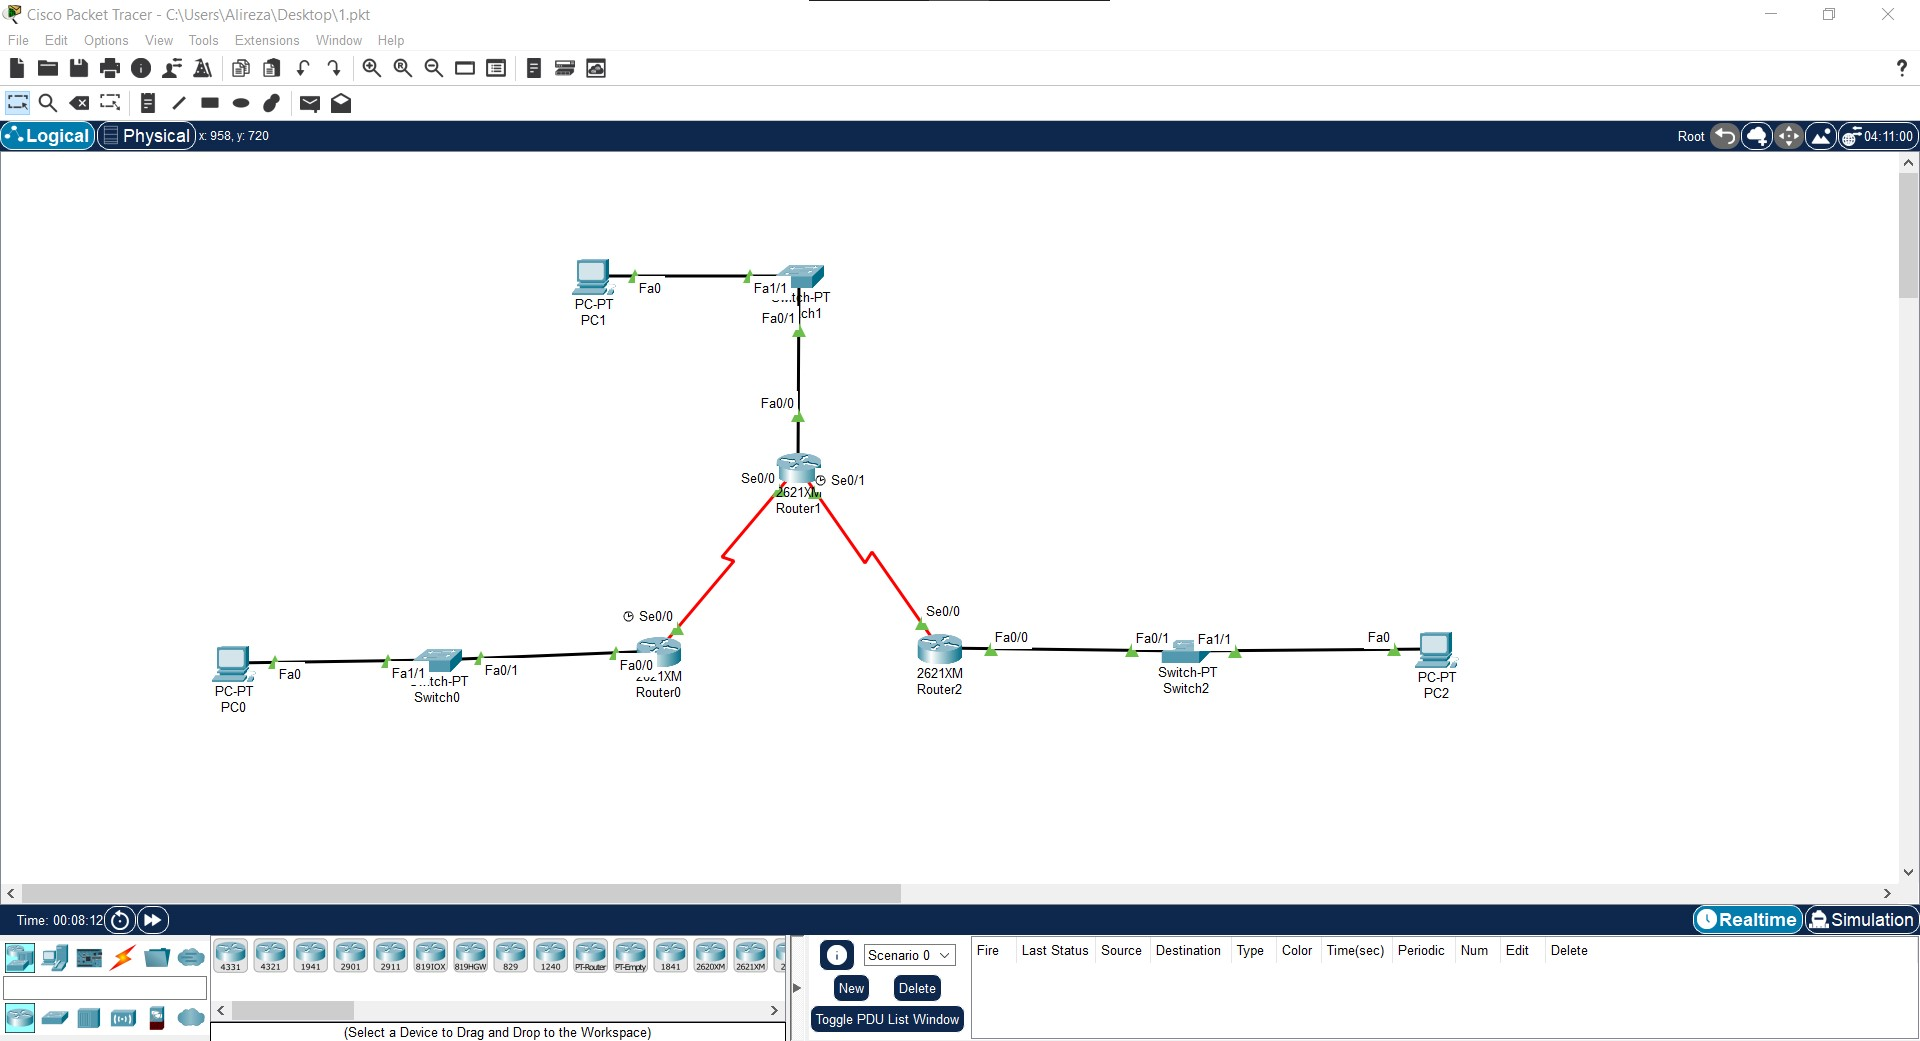
\includegraphics[width=1.0\textwidth]{figures/7.jpg}
    \caption{}
    \label{fig:fig1}
\end{figure}
\begin{figure}[H]
    \centering
    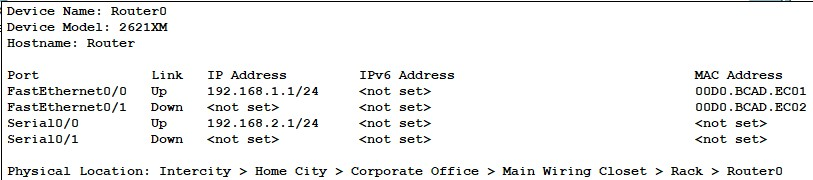
\includegraphics[width=0.5\textwidth]{figures/8.jpg}
    \caption{}
    \label{fig:fig1}
\end{figure}
\begin{figure}[H]
    \centering
    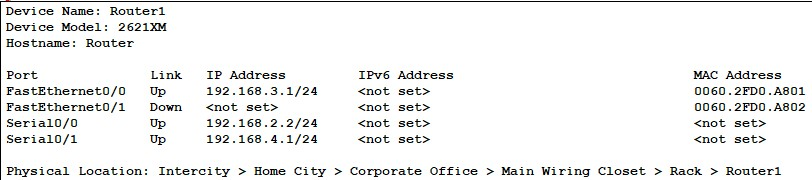
\includegraphics[width=0.5\textwidth]{figures/9.jpg}
    \caption{}
    \label{fig:fig1}
\end{figure}

\begin{figure}[H]
    \centering
    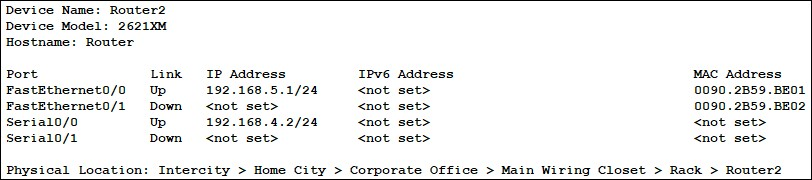
\includegraphics[width=0.5\textwidth]{figures/10.jpg}
    \caption{}
    \label{fig:fig1}
\end{figure}
حال باید \lr{PC}ها را کانفیگ کنیم. به این منظور به طریق زیر اقدام می‌کنیم.
\begin{figure}[H]
    \centering
    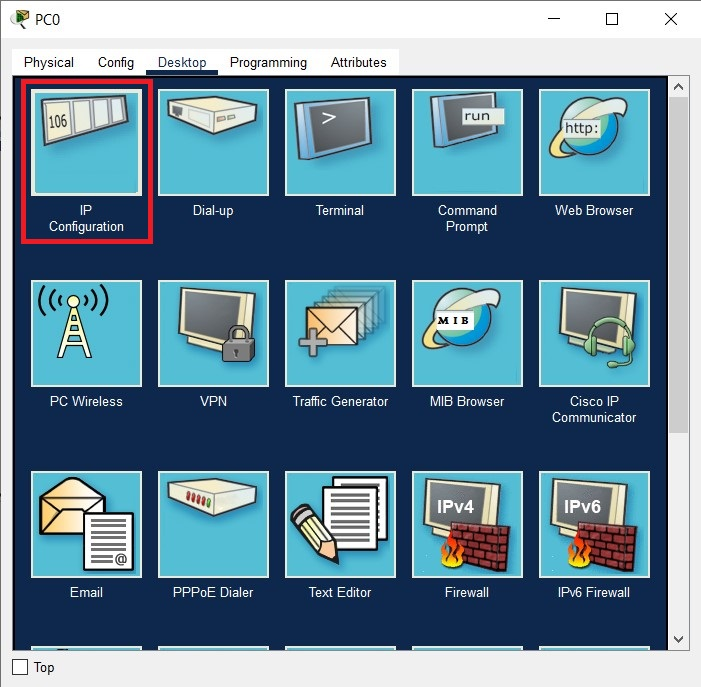
\includegraphics[width=0.75\textwidth]{figures/11.jpg}
    \caption{}
    \label{fig:fig1}
\end{figure}
\begin{figure}[H]
    \centering
    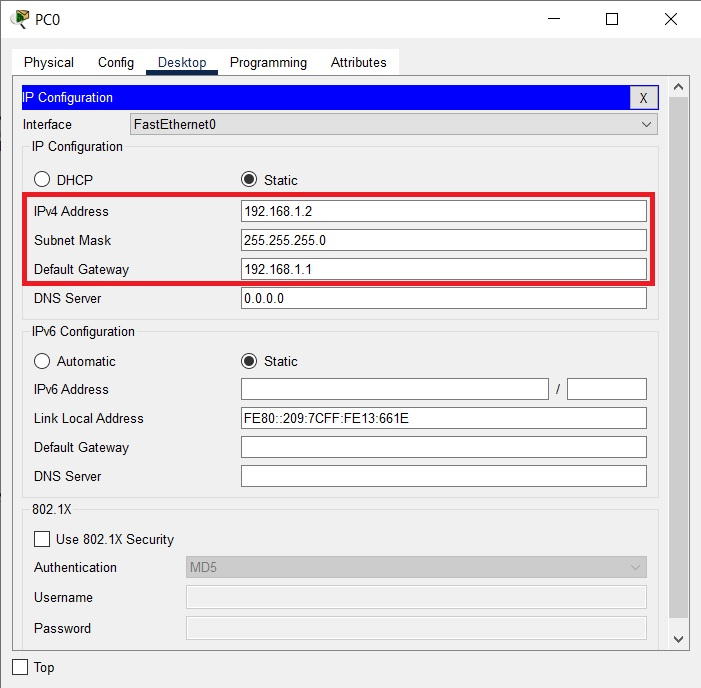
\includegraphics[width=0.75\textwidth]{figures/12.jpg}
    \caption{}
    \label{fig:fig1}
\end{figure}


\section{}%5
به شکل زیر وضعیت اینترفیس‌ها را بررسی می‌کنیم.
\begin{figure}[H]
    \centering
    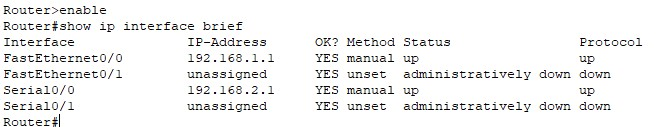
\includegraphics[width=0.5\textwidth]{figures/r2.jpg}
    \caption{}
    \label{fig:fig1}
\end{figure}
\begin{figure}[H]
    \centering
    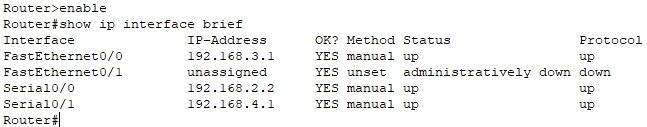
\includegraphics[width=0.5\textwidth]{figures/r3.jpg}
    \caption{}
    \label{fig:fig1}
\end{figure}
\begin{figure}[H]
    \centering
    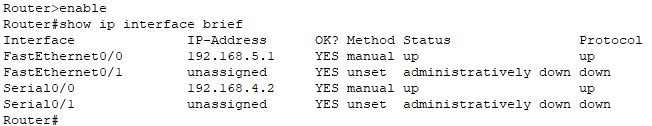
\includegraphics[width=0.5\textwidth]{figures/r4.jpg}
    \caption{}
    \label{fig:fig1}
\end{figure}

\section{}%6
\begin{figure}[H]
    \centering
    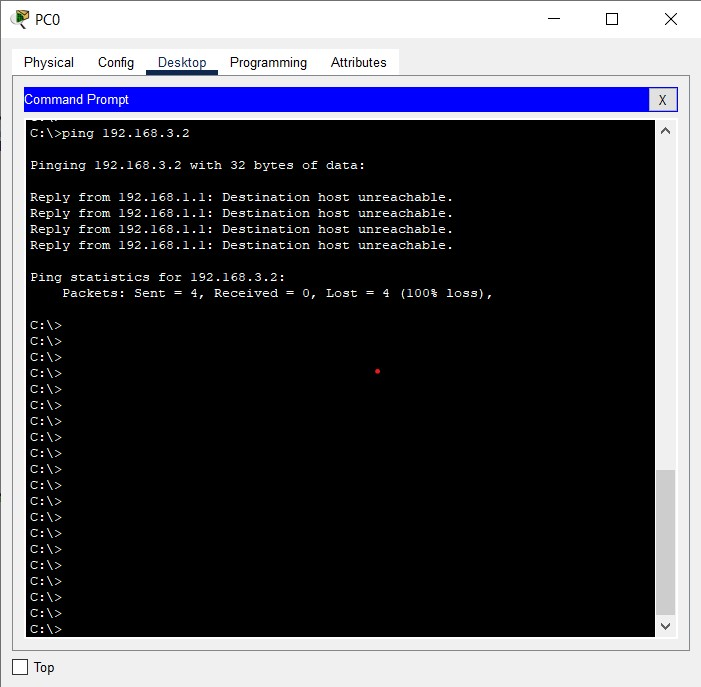
\includegraphics[width=0.75\textwidth]{figures/13.jpg}
    \caption{}
    \label{fig:fig1}
\end{figure}
همانطور که می‌بینیم \lr{PC0} به \lr{PC1} دسترسی ندارد. برای سایر \lr{PC}ها هم همین وضعیت برقرار است و اتصال برقرار نمی‌باشد. چون دیوایس‌ها در دو شبکه‌ی مختلف هستند و جدول مسیریابی برای روترها پیکربندی نشده است.



\section{}%7
\begin{figure}[H]
    \centering
    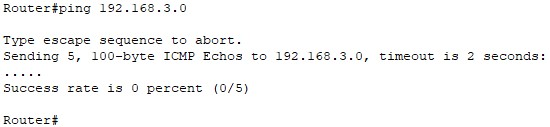
\includegraphics[width=0.75\textwidth]{figures/14.jpg}
    \caption{}
    \label{fig:fig1}
\end{figure}
به دلیل مشابه قسمت قبل روتر 0 (و سایر روترها) نمی‌تواند شبکه‌ی \lr{192.168.3.0} (یا شبکه‌های دیگر) را \lr{ping} کند و دسترسی وجود ندارد.

\section{}%8
به طریق زیر یک مسیر استاتیک بین دو شبکه‌ی \lr{192.168.1.0/24} و  \lr{192.168.3.0/24} برقرار می‌کنیم.
\begin{figure}[H]
    \centering
    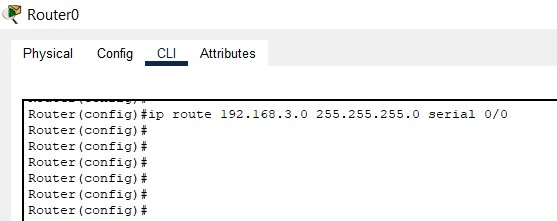
\includegraphics[width=0.75\textwidth]{figures/15.jpg}
    \caption{}
    \label{fig:fig1}
\end{figure}
\begin{figure}[H]
    \centering
    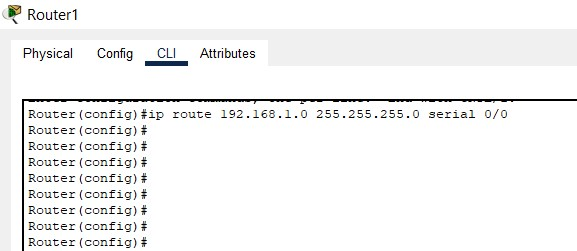
\includegraphics[width=0.75\textwidth]{figures/16.jpg}
    \caption{}
    \label{fig:fig1}
\end{figure}
سایر مسیرها را به طریق مشابه برقرار می‌کنیم.
\section{}%9
\begin{figure}[H]
    \centering
    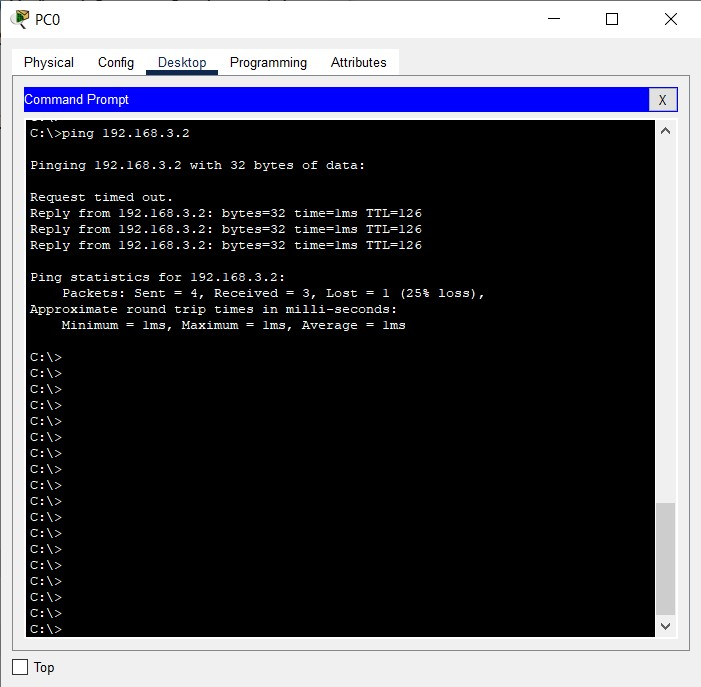
\includegraphics[width=0.75\textwidth]{figures/17.jpg}
    \caption{}
    \label{fig:fig1}
\end{figure}

\section{}%10
\begin{figure}[H]
    \centering
    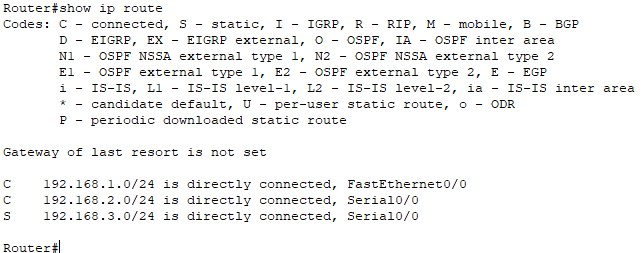
\includegraphics[width=0.75\textwidth]{figures/18.jpg}
    \caption{}
    \label{fig:fig1}
\end{figure}
\begin{figure}[H]
    \centering
    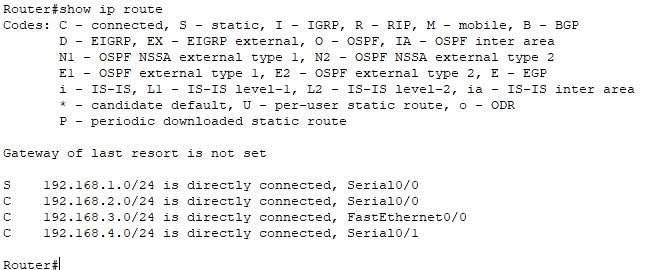
\includegraphics[width=0.75\textwidth]{figures/19.jpg}
    \caption{}
    \label{fig:fig1}
\end{figure}

\section{}%11
\begin{figure}[H]
    \centering
    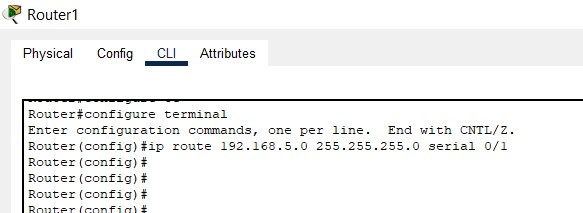
\includegraphics[width=0.75\textwidth]{figures/20.jpg}
    \caption{}
    \label{fig:fig1}
\end{figure}
\begin{figure}[H]
    \centering
    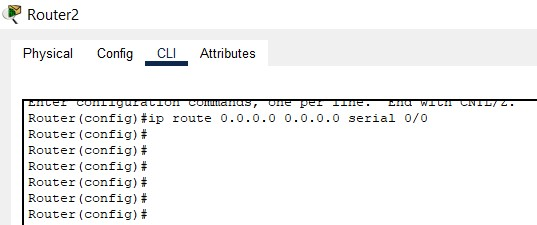
\includegraphics[width=0.75\textwidth]{figures/21.jpg}
    \caption{}
    \label{fig:fig1}
\end{figure}

\section{}%12
\begin{figure}[H]
    \centering
    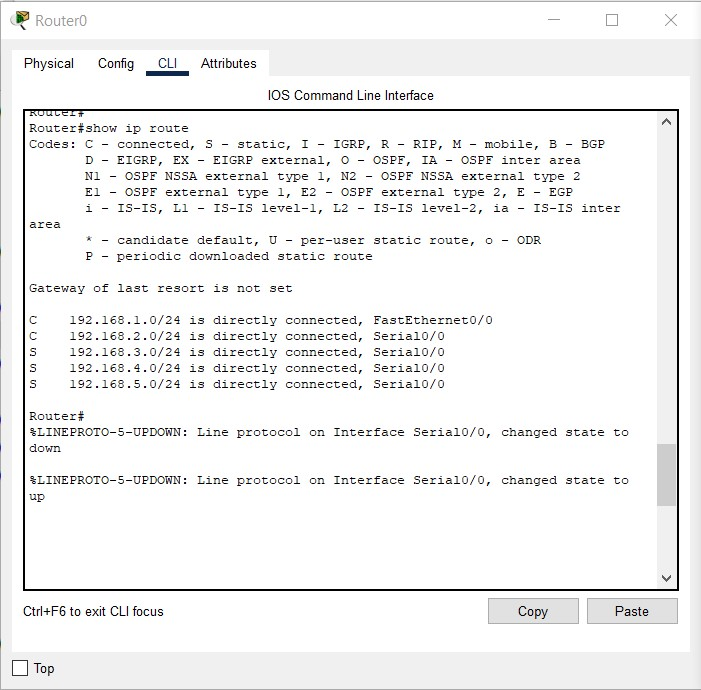
\includegraphics[width=0.75\textwidth]{figures/22.jpg}
    \caption{}
    \label{fig:fig1}
\end{figure}
\begin{figure}[H]
    \centering
    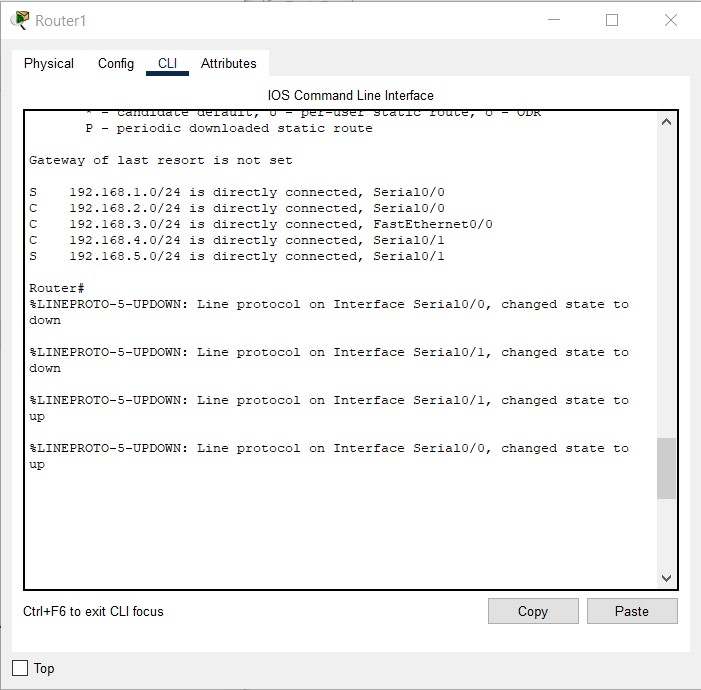
\includegraphics[width=0.75\textwidth]{figures/23.jpg}
    \caption{}
    \label{fig:fig1}
\end{figure}
\begin{figure}[H]
    \centering
    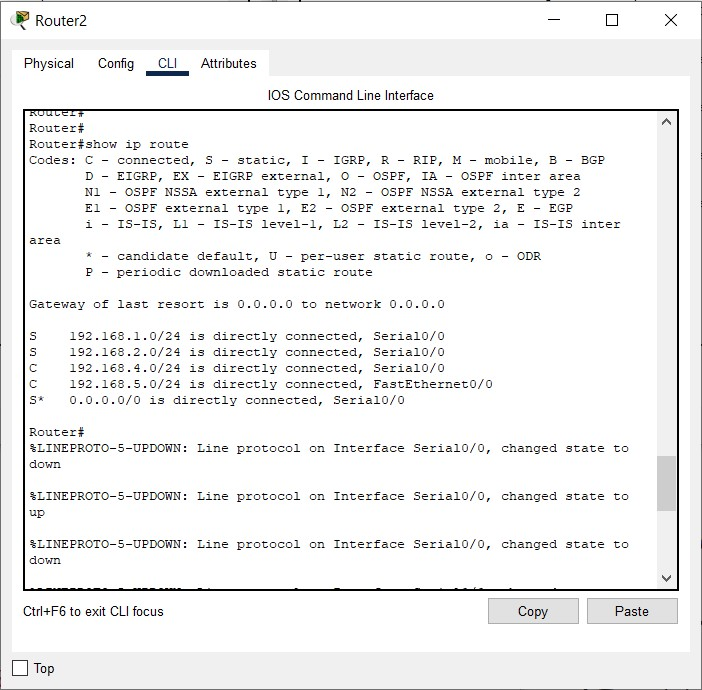
\includegraphics[width=0.75\textwidth]{figures/24.jpg}
    \caption{}
    \label{fig:fig1}
\end{figure}
\section{}%13
در \lr{Default Route} می‌توان یک مسیر پیش‌فرض تعریف کرد. در اینصورت اگر بسته‌ای وارد مسیریاب گردد که با هیچ یک از مسیرهای جدول مسیریابی همخوانی نداشته باشد، به این مسیر هدایت می‌گردد. در حقیقت این مسیر با هر آدرس شبکه‌ای همخوانی دارد. اما در مسیریابی استاتیک پورت خروجی به ازای هر مقصد باید به طور خاص پیکربندی شود.
\section{}%14
\begin{figure}[H]
    \centering
    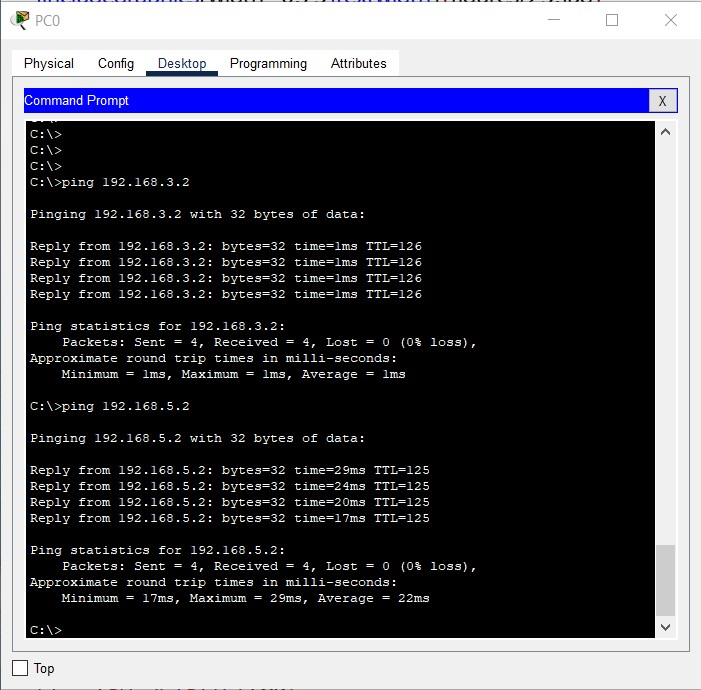
\includegraphics[width=0.75\textwidth]{figures/25.jpg}
    \caption{}
    \label{fig:fig1}
\end{figure}
\begin{figure}[H]
    \centering
    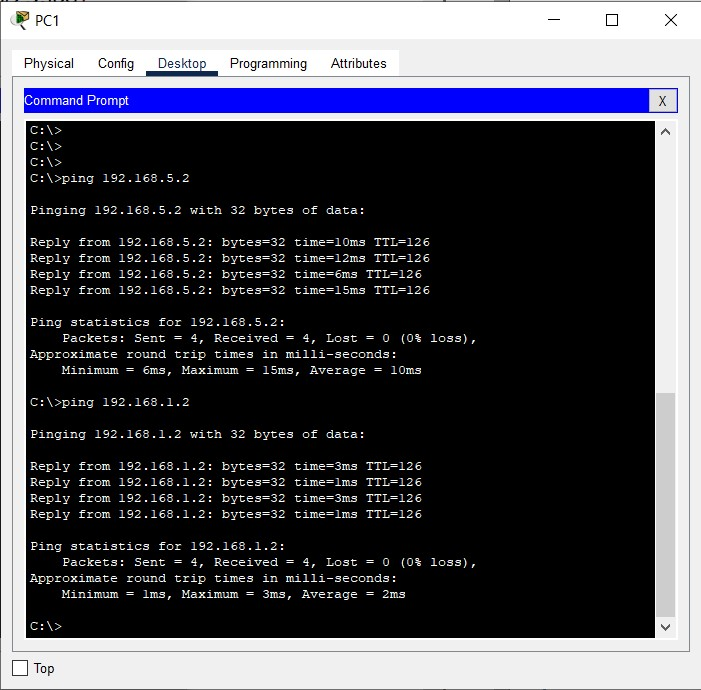
\includegraphics[width=0.75\textwidth]{figures/26.jpg}
    \caption{}
    \label{fig:fig1}
\end{figure}
\begin{figure}[H]
    \centering
    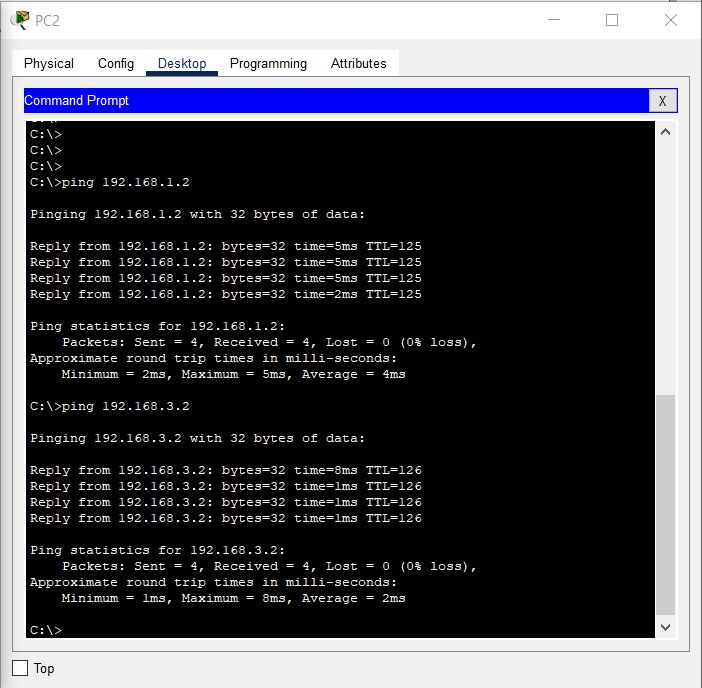
\includegraphics[width=0.75\textwidth]{figures/27.jpg}
    \caption{}
    \label{fig:fig1}
\end{figure}
از آنجایی جدول مسیریابی برای هر 5 شبکه در همه روترها فیکس شده است، پس ارتباط بین همه عناصر شبکه برقرار است.
\section{}%15

\subsection{روتر 0}
\begin{latin}
\VerbatimInput{source/rt0.txt}
\end{latin}
\subsection{روتر 1}
\begin{latin}
\VerbatimInput{source/rt1.txt}
\end{latin}
\subsection{روتر 2}
\begin{latin}
\VerbatimInput{source/rt2.txt}
\end{latin}

\section{}%16
با استفاده از دستور \lr{copy running-config startup-config} یا \lr{write mem} تنظیمات را ذخیره می‌کنیم.




%%%%%%%%%%%%%%%%%%%%%%%%%%%%%%%%%%%%%%%%%%%%%%

\section*{منابع}
\renewcommand{\section}[2]{}%
\begin{thebibliography}{99} % assumes less than 100 references
%چنانچه مرجع فارسی نیز داشته باشید باید دستور فوق را فعال کنید و مراجع فارسی خود را بعد از این دستور وارد کنید


\begin{LTRitems}

\resetlatinfont

\bibitem{b1}
\end{LTRitems}

\end{thebibliography}


\end{document}
